The HF is located at 11.3 m from the interaction point and provides a
pseudo-rapidity coverage from $|\eta|>3.0$ to $|\eta|<5.2$. Since
there is no coverage from the tracker or ECAL in this region, the energy deposited in HF
is used to reconstruct forward jets and also to calculate
\ptmiss. Hence a stable performance of HF is important both for SM
measurements and new physics searches.

The quartz fibers are inserted into the steel absorber plates. Half
of the fibers run over the full depth of the HF (165 cm $\approx$ 10
interaction lengths) while the remaining half of the fibers start at a
depth of 22 cm from the front face of the detector. The former
are called {\bf long fibers} and latter are called {\bf short
  fibers}. The energies deposited in long and short fibers are read
out separately, and are called {\elong} and {\eshort} respectively.

The signal in HF is due to the Cherenkov light produced by charged particles as they traverse through the quarts fibers. The
Cherenkov light is emitted only when the particle's velocity is greater than the speed of light in that medium. If the particle has sufficient energy, it can travel faster than light in that medium and produce Cherenkov light. This light is collected by the long and short optical fibers. The recordable signal in calorimeter is due to the electromagnetic and hadronic component of the particle showers. Since electrons or photons result in shorter showers, these result in signal mostly
in long fibers. The hadronic showers, however, continue deeper and
result in signal in both long and short fibers.

The ratio of energy measured in short and long fibers,
\ratiosl = \eshort/\elong, depends on the energy of the incident
particle which created the shower and hence on how deeply the shower
has penetrated the calorimeter. However, the average \ratiosl
over a period of time in a given $\eta$ region is expected
to depend on average energy incident on the calorimeter and
accelerator run conditions (which determines the pileup, the number of pp interactions). In this
section, we describe studies \ratiosl for data collected at $\sqrt{s} = 8$
TeV and  $\sqrt{s} = 13$ TeV, and also the effect of pileup. 
Since the average \ratiosl for various channels of a
given $i\eta$ ring is expected to be same, this quantity can
be used to intercalibrate the short fibers across $\phi$
while the long fibers are calibrated using Z$\rightarrow e^+e^-$ events.

\subsection{Data and simulation samples}\label{sec:dataset}
These studies make use of data collected by CMS detector in the years 2012, 2015 and 2016.
Each of these are divided into different parts and they are named by adding a suffix to the year,
for example 2012D is a subset of data collected in 2012. The events from these dataset are selected
using triggers which are based on hadronic activity, calculated using sum \pt of all jets or using 
highest \pt jet in the event. The dataset which contains hadronic triggers is called as \textit{JetHT} dataset. 
Only those data which are certified as good for physics analysis are used. 
Table \ref{tab:dataSamples} shows list of datatsets used for this study along with pp bunch spacing and integrated 
luminosity of the dataset.
Monte-carlo (MC) simulated sample consists of QCD events generated at
leading order (LO) taking $\sqrt{s}=13$ TeV using MadGraph generator and hadronization is carried out using Pythia8.

\begin{table}[!h]
\centering
\caption[Collision data used for \ratiosl studies of HF]{Collision data used for \ratiosl studies of HF. The 2012 data were taken at $\sqrt{s}=8$ TeV and all other data were taken at $\sqrt{s}=13$ TeV.}
\label{tab:dataSamples}
\begin{tabular}{lccc}
\hline
Data	&	Bunch spacing (ns) 	& \lumi \ (\pbinv)\\\hline\hline
2012D	&	50					&	962 \\\hline
2015B	&	\multirow{2}{*}{50}	&	40.9\\
2015C	&						&	25.0\\ \hline
2015C	&	\multirow{2}{*}{25}	&	16.3\\
2015D	&						&	$1.61\times 10^3$\\\hline
2016B	&	\multirow{7}{*}{25}	&	$5.28\times 10^3$\\
2016C	&						&	$789$\\
2016D	&						&	$3.28\times 10^3$\\
2016E	&						&	$4.05\times 10^3$\\
2016F	&						&	$3.11\times 10^3$\\
2016G	&						&	$7.11\times 10^3$\\
2016H	&						&	$8.68\times 10^3$\\\hline
\end{tabular}
\end{table}

%\graphicspath{{/home/vinay/work/HFanalysisLocal/TreeMakerFiles/AnalysisNote/}}
\subsection{Energy in long and short fibers of HF}
The HF starts at $|\eta|$=2.853 and extends up to $|\eta|$=5.191. On 
both the $\pm z$ sides, this $\eta$ range is divided into 13 towers 
with tower index starting from $i\eta$=29 and ending at $i\eta$=41. 
Towers $|i\eta|$=29 to $|i\eta|$=39 have 36 divisions ($10^\circ$ each) 
in $\phi$ and towers $|i\eta|$=40 and 41 have 18 
divisions ($20^\circ$ each). In total there are 864 channels. Depth 
segment with index 1 corresponds to long fibers and depth segment
with index 2 refers to short fibers in each of these channels.
If the energy in a particular channel is above the noise level, then that channel is 
considered to have a \textit{rechit} (recorded hit).

All the plots and discussion till the end of section \ref{pileup} correspond to 2015C-50ns data.
\begin{itemize}
\item Fig.~\ref{fig:254833_ietavsIphiD1D2} shows a typical distribution of number of rechits, with rechit energy $>$ 10\,GeV, in each of the channels in depth 1 (long fibers) and depth 2 (short fibers). 
\begin{figure}[h!]
\begin{minipage}[b]{0.5\linewidth}
\centering
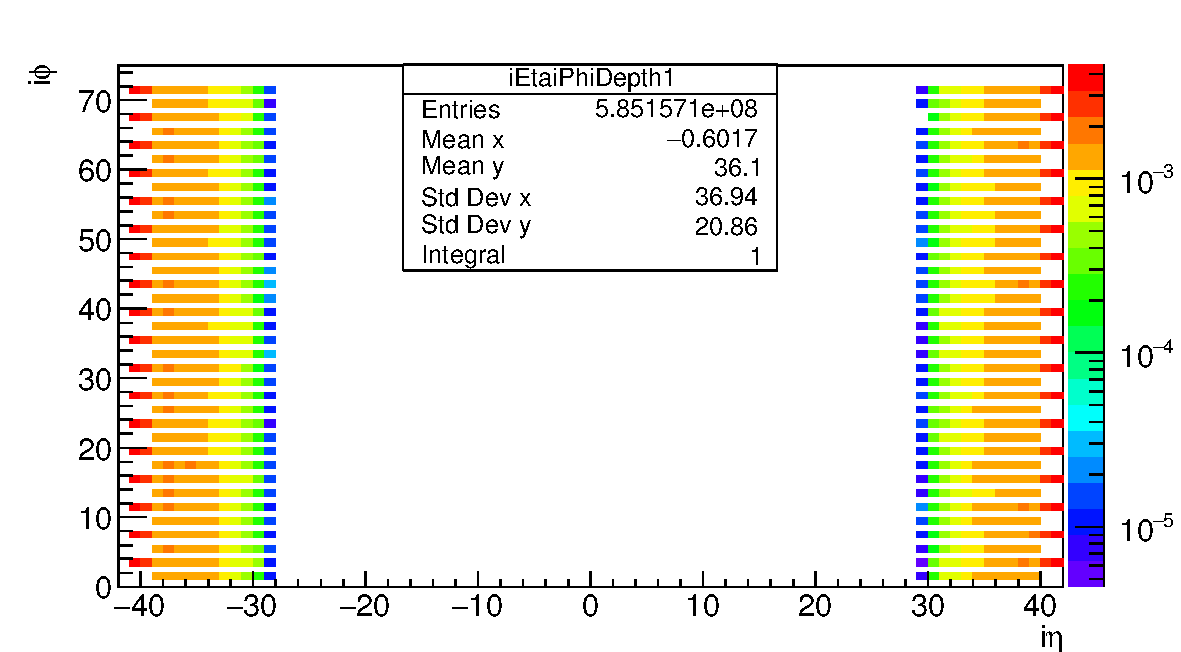
\includegraphics[width=.99\linewidth]{../Figures/Chap2/ImageFiles_HF/BasicPics/254833_ietavsIphiD1.pdf}
%\caption{Number of RecHits in depth 1}
%\label{fig:254833_ietavsIphiD1}
\end{minipage}
%\hspace{0.1cm}	
\begin{minipage}[b]{0.5\linewidth}
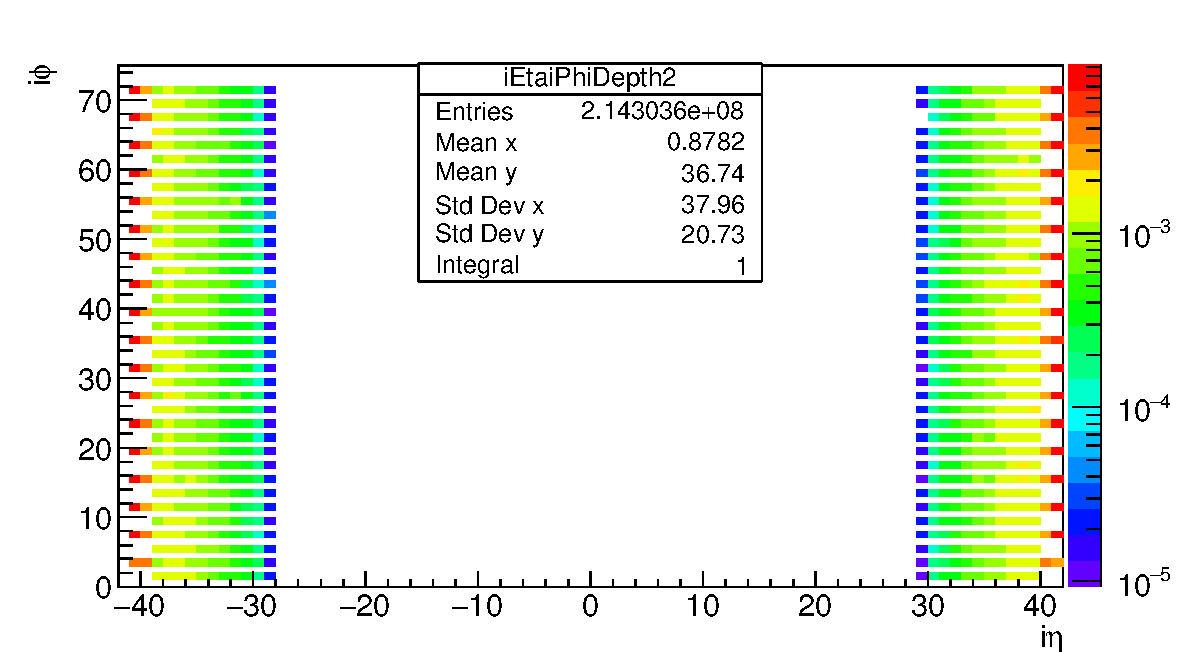
\includegraphics[width=0.99\linewidth]{../Figures/Chap2/ImageFiles_HF/BasicPics/254833_ietavsIphiD2.pdf}
%\caption{Channel occupancy for (left) depth 1, and (right) depth 2.}
%\label{fig:254833_ietavsIphiD1D2}
\end{minipage}
\caption{Channel occupancy for depth 1 (left), and depth 2 (right).}
\label{fig:254833_ietavsIphiD1D2}
\end{figure}

\item Fig.~\ref{fig:nRecHits} shows the total number of rechits 
distribution inclusive in $i\eta$ and $i\phi$ with rechit energy 
$>$10 GeV.
\begin{figure}[h!]
\centering
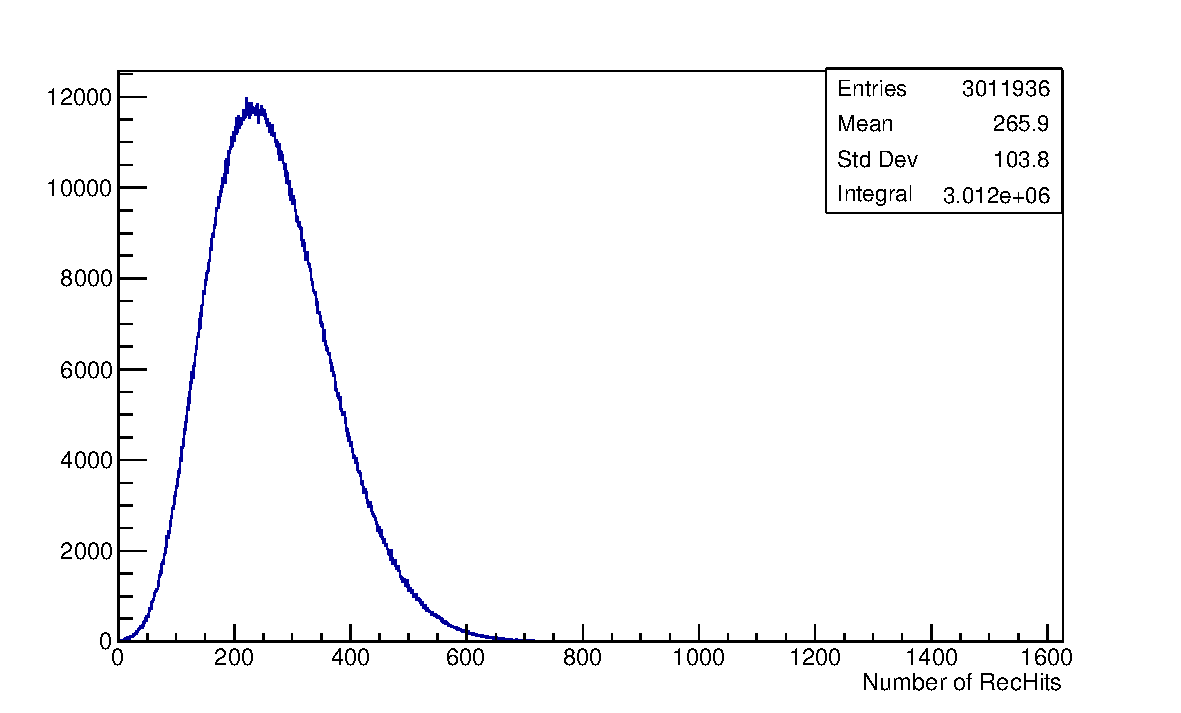
\includegraphics[width=0.5\linewidth]{../Figures/Chap2/ImageFiles_HF/BasicPics/nRecHits.pdf}
\caption{Total number of rechits (inclusive in $i\eta$ and $i\phi$) }
\label{fig:nRecHits}
\end{figure}
\item Fig.~\ref{fig:EsvsElNoECut} shows the energy distribution in 
short fibers (\eshort) vs long fiber (\elong) without any threshold
on their recorded energies. This figure shows that there is correlation 
between \elong and \eshort. So we use \ratiosl as a tool for studying 
the performance of HF.

There two more important points to note from this plot: firstly, there
are cases with a large \elong while there is almost no energy deposited 
in corresponding short fiber i.e. \eshort$<$ 10 GeV. This can be due to EM showers. Secondly, there are
cases when there is large energy deposited in short fibers while small
energies in long fibers (\elong$<$30 GeV). It is not expected to have 
large energy deposits in only one of the fibers if the shower originates
from hadrons. One of the reasons for this could be that some of the 
high energy particles directly hit the glass window of PMT and resultant Cherenkov light produced in the glass gives rise
to a large signal in only one of the channels. To reject such hits, 
thresholds are placed on reconstructed energies of rechits, \eshort$>10~$\gev
and \elong$>40~$\gev. From this point onwards, one can assume that these 
threshold have been applied on \eshort and \elong unless a different 
selection is explicitly mentioned.

\begin{figure}[h!]
\centering
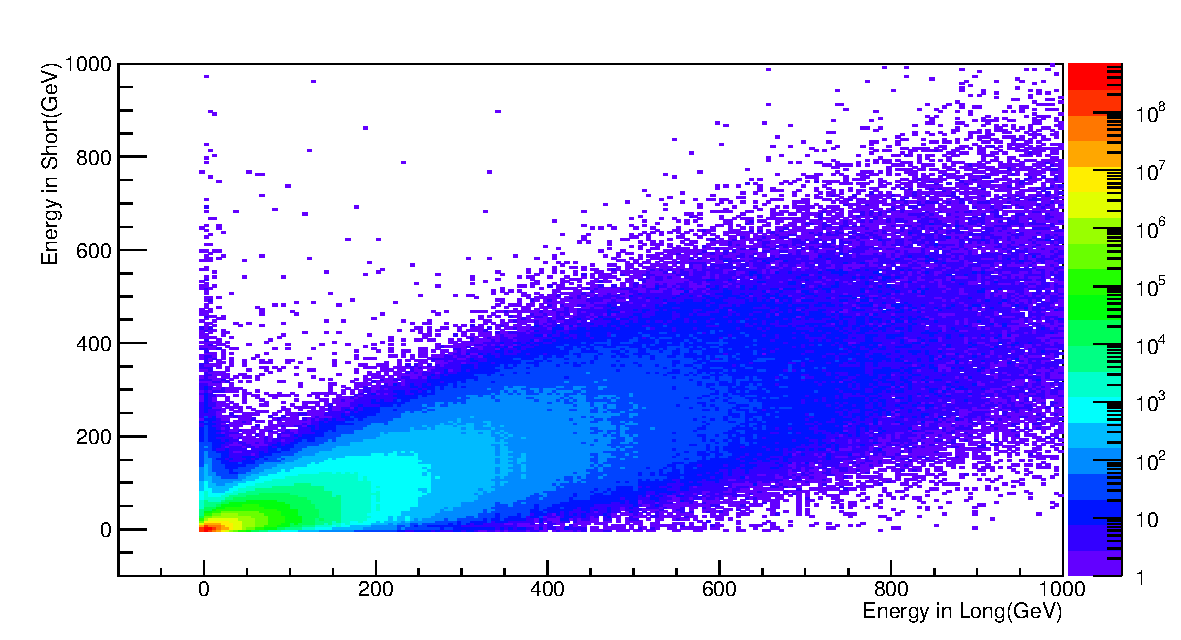
\includegraphics[width=0.7\linewidth]{../Figures/Chap2/ImageFiles_HF/BasicPics/EsvsElNoECut.pdf}
\caption{Distribution of \eshort vs \elong for HF channels.}
\label{fig:EsvsElNoECut}
\end{figure}

\item With the energy thresholds mentioned above, \ratiosl is studied 
for each $i\eta$ tower. The Fig.\ref{1DRatio} shows distribution of
the \ratiosl for the tower $i\eta=$32 integrated over all $i \phi$ 
channels. Since the mean value of the distribution is sensitive to 
the tails, we try to fit it with an asymmetric Gaussian 
 (eqn.\ref{asymGaus}) and use the peak value obtained from the fit
to indicate the average ratio for a given $i\eta$ ring.

\begin{figure}[h!]
\centering
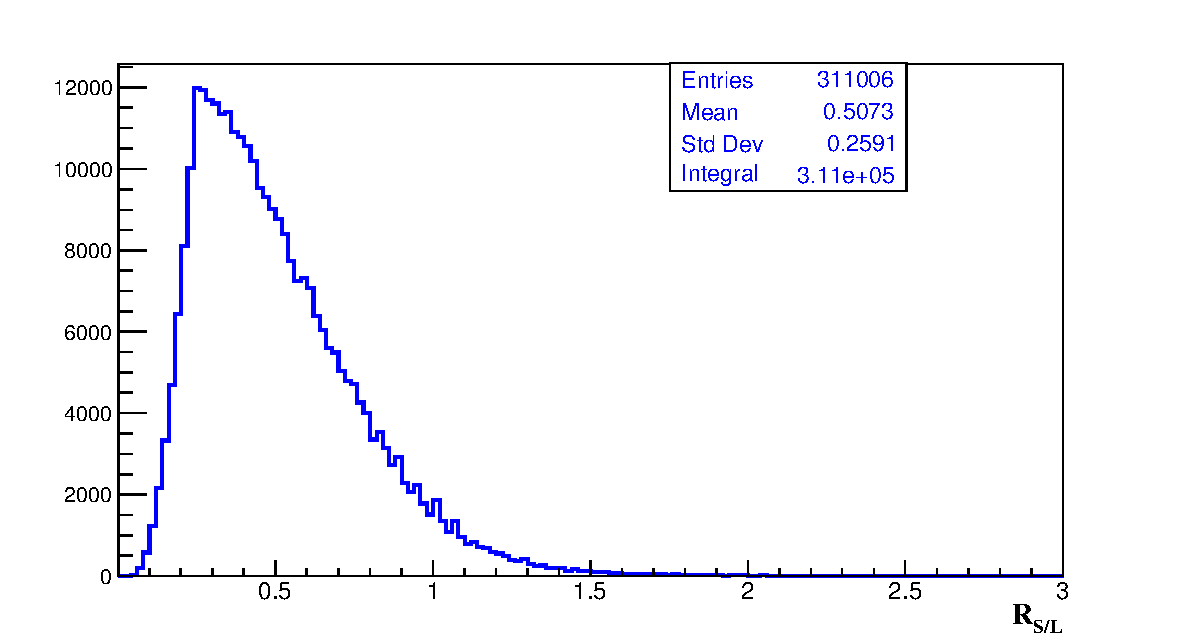
\includegraphics[width=0.7\linewidth]{../Figures/Chap2/ImageFiles_HF/Ratio/Ratioieta32254833El40.pdf}
\caption{\ratiosl for $i \eta\ 32$ tower with $i \phi$ inclusive for 2015D-50 ns.}
\label{1DRatio}
\end{figure}
\begin{equation}
f(x)=e^{-\frac{(x-\mu)^2}{2\sigma^2}}\left[ 1+erf\left( \frac{x-\mu}{\sqrt{2}\sigma}\right) \right] 
\label{asymGaus} 
\end{equation}
Fitting the \ratiosl with an asymmetric Gaussian works very well for 
smaller $i\eta$ channels (Fig.~\ref{goodfit}). For the channels in
higher $i\eta$ regions, fitting does not work well and $\chi^2/dof$ is 
very large (Fig.~\ref{badfit}). Changing the fit range did not improve the fits significantly. So using the peak obtained from the 
fits cannot be used for studying all the channels. We then use 90\% 
truncated mean of the distribution - starting from the arithmetic peak,
bin contents are added on both the sides until the total integral is
90\% of the total area under the curve. From this point onward, mean 
refers to 90\% truncated mean. 
%\textcolor{red}{Comparison between arithmetic mean, 
%truncated mean and the peak obtained from the fit for different 
%$i\eta$ are shown in appendix~\ref{AppendixA} Fig.~\ref{MeanvsFit}.
%Fits for all the $i\eta$ towers are shown in appendix~\ref{AppendixA}
%Figs.~\ref{fig:Ratioieta29to32} to \ref{fig:Ratioieta41}.}

\begin{figure}[ht]
\begin{minipage}[b]{0.45\linewidth}
\centering
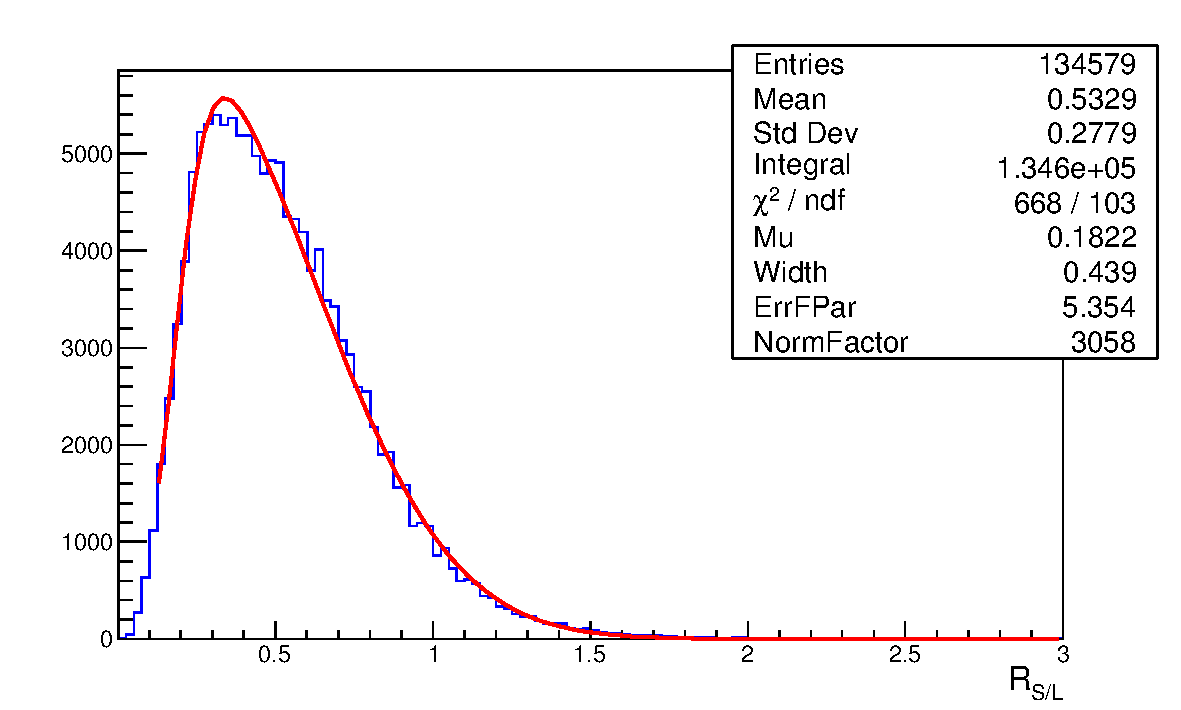
\includegraphics[width=\textwidth]{../Figures/Chap2/ImageFiles_HF/Ratio/RatioietaP30.pdf}
\captionsetup{width=.9\linewidth}
\caption{Asymmetric Gaussian fit for $i \eta$ 30}
\label{goodfit}
\end{minipage}
\hspace{0.5cm}
\begin{minipage}[b]{0.45\linewidth}
\centering
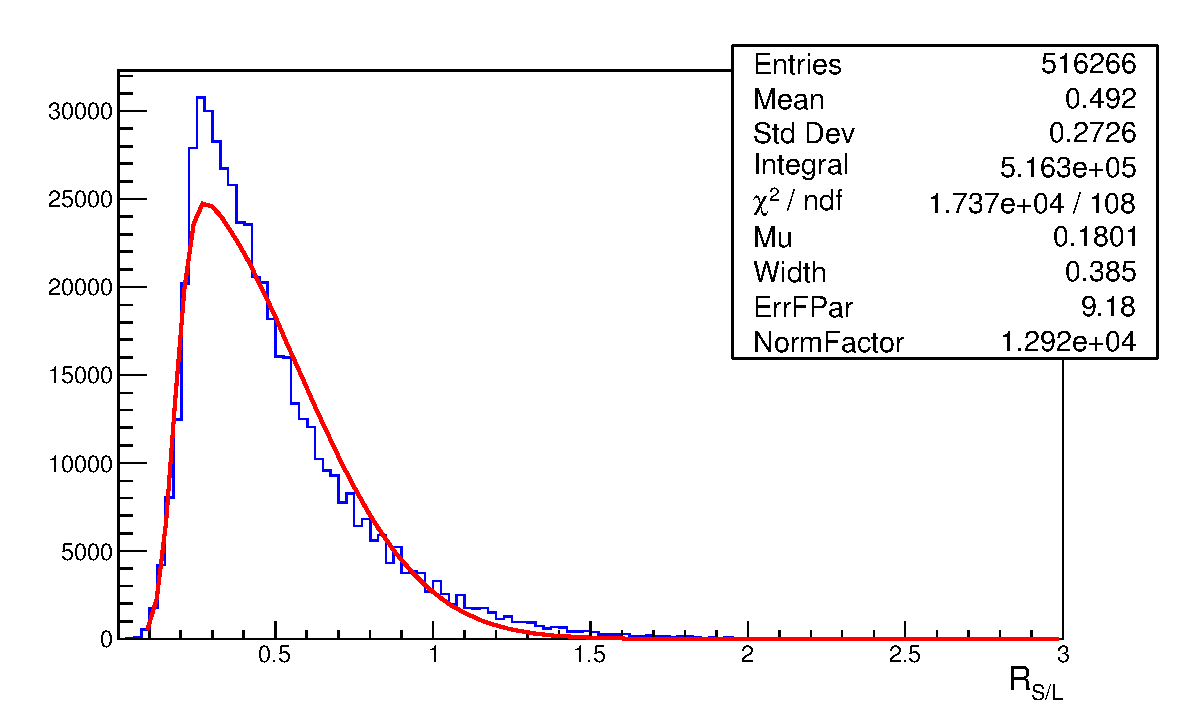
\includegraphics[width=\textwidth]{../Figures/Chap2/ImageFiles_HF/Ratio/RatioietaP39.pdf}
\captionsetup{width=.9\linewidth}
\caption{Asymmetric Gaussian fit for $i \eta$ 39}
\label{badfit}
\end{minipage}
\end{figure}

\subsection{Effect of Pileup on \ratiosl}\label{pileup}
The \ratiosl was studied under different pileup (PU) scenarios. If the number 
of good primary vertices is less than 9, it is considered as low pileup; 
between 11 and 16 as medium pileup and above 18 as high pileup.\\
Pileup is mainly dominated by low energy particles
and these particles do not have enough energy to penetrate into the short fibers and hence they deposit energy mainly in long fibers.
Hence these particles give lower \ratiosl than the high energy particles. Pileup is added on top of
a hard scattered events, and in hard scattered event \ratiosl is higher than PU events. Thus 
with increase of more and more pileup events, the \ratiosl is decreasing and that is the observation. With the high pileup, average energy deposits in long fibers is expected 
to be higher and as a result the \ratiosl is expected to be lower as 
compared to the low pileup scenario.Fig.~\ref{RvsIetaComparePileups} shows 
that higher pileup means lower ratio and lower pileup means higher ratio. 
The shaded region corresponds to all events wherein no restriction on pileup is 
applied.

\begin{figure}[h!]
\centering
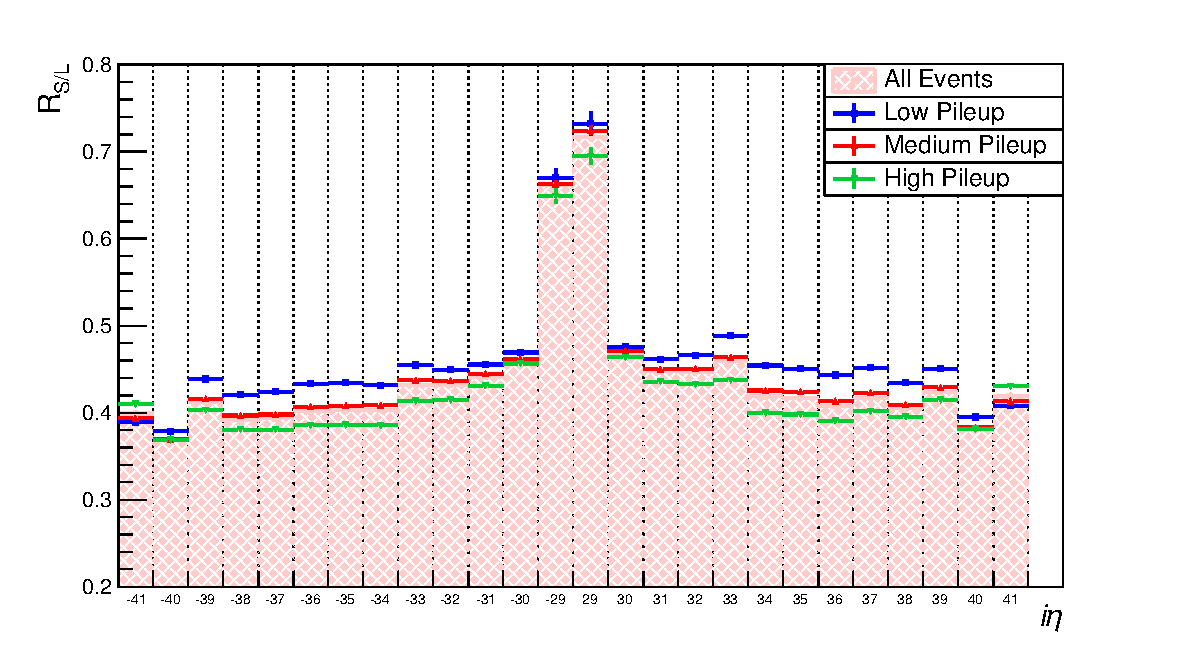
\includegraphics[width=0.7\linewidth]{../Figures/Chap2/ImageFiles_HF/Ratio/RvsIetaComparePileups.pdf}
\captionsetup{width=.9\linewidth}
\caption{Effect of pileup on \ratiosl for different $i\eta$ rings (integrated over $i\phi$ channels.}
\label{RvsIetaComparePileups}
\end{figure}

\end{itemize}


\subsection{Studying \ratiosl at $\sqrt{s}=$13 TeV and 8 TeV data with 50 ns bunch spacing}\label{sec:ana50ns}

\begin{itemize}
\item In 2015, LHC started 13 TeV collisions with 50 ns bunch spacing. We compared \ratiosl for 13 TeV data taken in 2015 and 8 TeV data taken in 2012.
\item Used JetHT dataset for 13TeV data and 8 TeV with all the events (no trigger based selection of events) for this study.
\item Average pile up was similar (Fig.\ref{fig:nVertices}) in 8 and 13 TeV datasets.

\begin{figure}[h!]
\centering
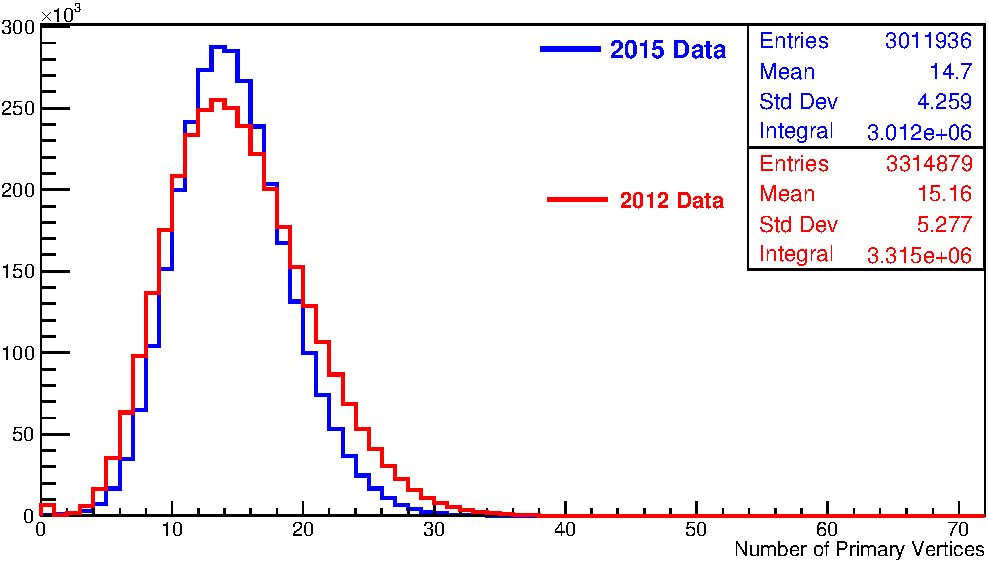
\includegraphics[width=0.7\linewidth]{../Figures/Chap2/ImageFiles_HF/2012vs2015/nVertices.pdf}
\caption{Pileup comparison for 2015 data and 2012 data}
\label{fig:nVertices}
\end{figure}

\item Fig.~\ref{2012vs2015E1} and \ref{2012vs2015E2} show the distributions of energies in long and short fibers, for 2012D and 2015C, with \elong, \eshort $>10~$\gev.

\begin{figure}[ht]
\begin{minipage}[b]{0.5\linewidth}
\centering
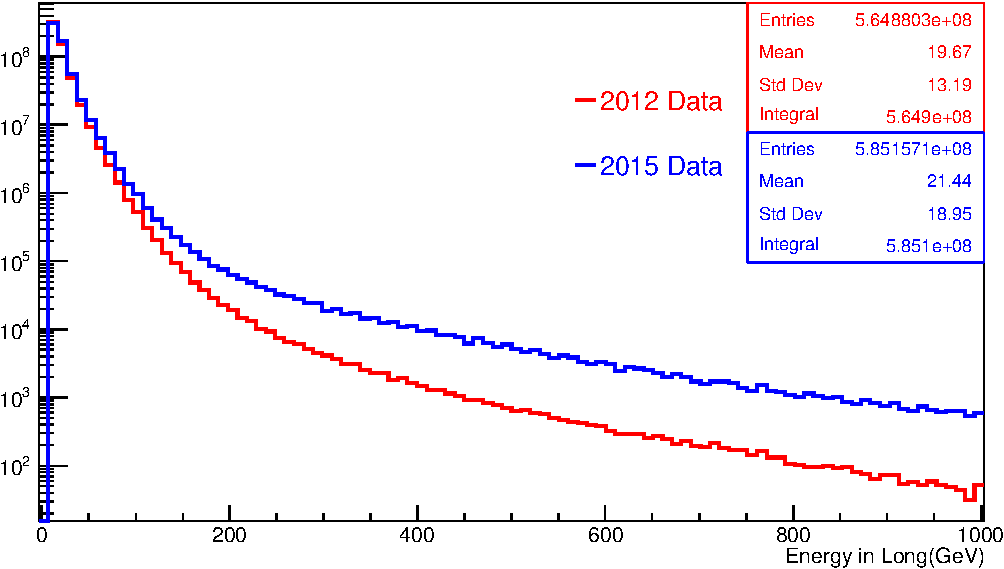
\includegraphics[width=\linewidth]{../Figures/Chap2/ImageFiles_HF/2012vs2015/Elong1DCompare.pdf}
\captionsetup{width=.9\linewidth}
\caption{Energy in long fibers}
\label{2012vs2015E1}
\end{minipage}
\hspace{0.5cm}
\begin{minipage}[b]{0.5\linewidth}
\centering
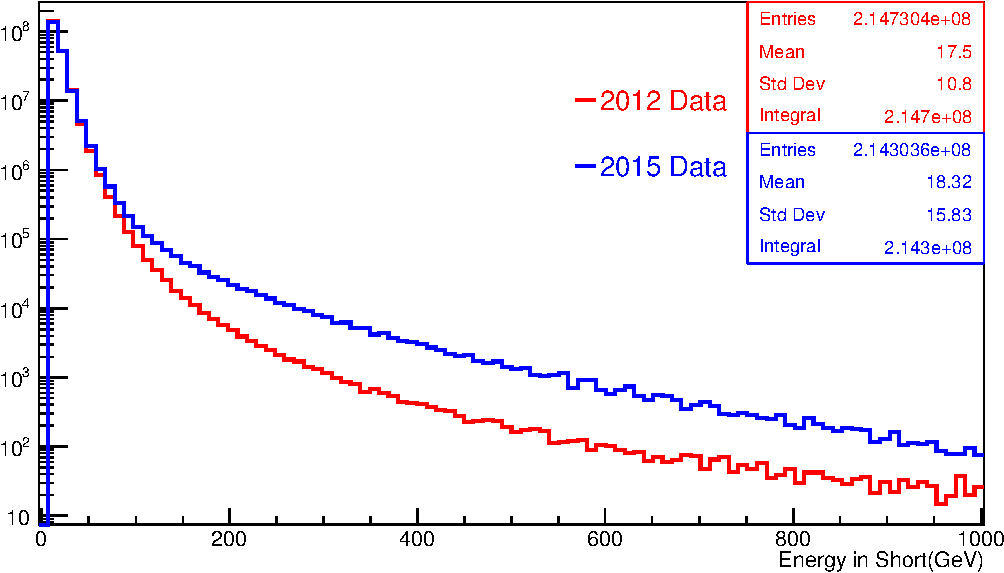
\includegraphics[width=\linewidth]{../Figures/Chap2/ImageFiles_HF/2012vs2015/Eshort1DCompare.pdf}
\captionsetup{width=.9\linewidth}
\caption{Energy in short fibers}
\label{2012vs2015E2}
\end{minipage}
\end{figure}
\end{itemize}

In 2015 p-p collisions, the $\sqrt{s}$ was 13 TeV and in 2012 it was only 8 TeV. 
Because of the increased energy of the collisions, the outgoing particles will have 
higher energy and hence these particles can penetrate deeper into the calorimeter giving
larger energy in short fibers. So the \ratiosl is expected to be higher in 13 TeV data as
compared to 8 TeV data. \ratiosl was determined for different $i \eta$ towers,with $i \phi$ 
inclusive and it was compared for 2012D data, 2015B data and 2015C data (fig, \ref{RvsIeta}).
For most of the $i \eta$ towers, \ratiosl of 2015 data is higher than that of 2012. With the 
increase of $\sqrt{s}$, average energy of particles is also increasing, consequently the 
\ratiosl is increasing. The reason for differences in 2015 and 2012 data could be because
of increased beam energy in p-p collisions and (or) the response of the fibers has changed.
\ratiosl for $|i\eta|$ 29 is much higher as compared to other $|i\eta|$ towers. This is because, this tower is behind $|i\eta|$ 28 of HE. EM shower energy is already deposited in HE. HF receives only hadronic shower energy and this energy is deposited in both long and short. Hence \ratiosl is higher for these towers.
\begin{figure}[h!]
\centering
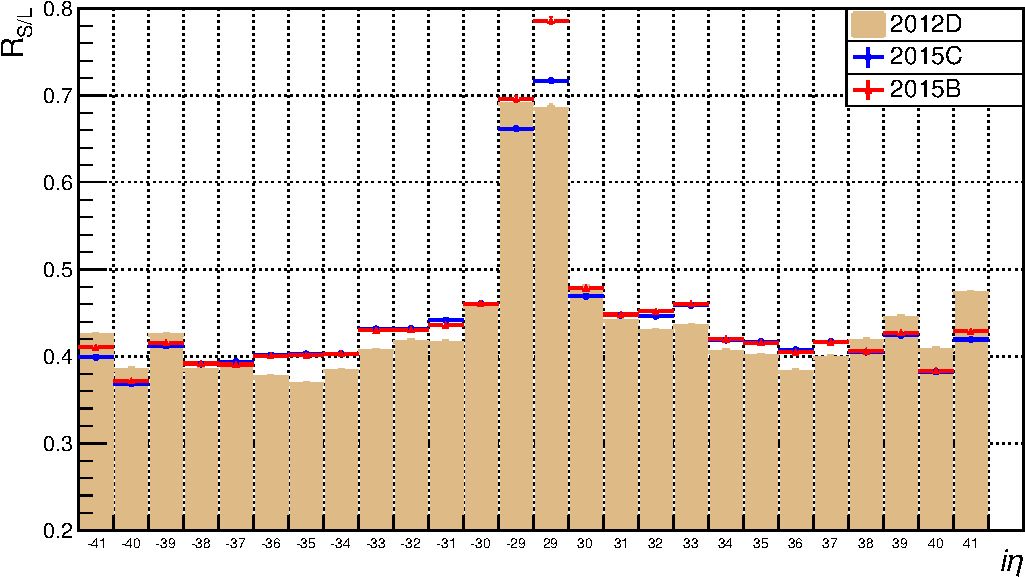
\includegraphics[width=0.7\linewidth]{../Figures/Chap2/ImageFiles_HF/2012vs2015/RvsIeta.pdf}
\caption{\ratiosl vs $i \eta$ for 3 different run conditions}
\label{RvsIeta}
\end{figure}
\ratiosl as a function of $i\phi$ for each $i \eta$ was also studied. Fig.~\ref{fig:Rvsiphi1} shows \ratiosl vs $i \phi$ for $i \eta$ -35. From this plot one can see whether a particular channel is problematic or not. In this figure, channel with $i \phi$ index 35 shows very high ratio in 2015B run. Also in most of the $i \phi s$, \ratiosl for 2012 data is slightly lower than 2015 data \ratiosl. %\textcolor{red}{The plots corresponding to each $i \eta$ is shown in Fig.\ref{fig:ieta29_32_E1E2Cut2Ietaiphi}-\ref{fig:ieta41E1E2Cut2Ietaiphi}  in appendix \ref{AppendixA}.}
\begin{figure}[h!]
\centering
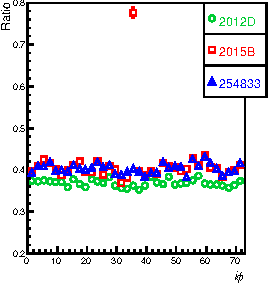
\includegraphics[width=0.5\linewidth]{../Figures/Chap2/ImageFiles_HF/2012vs2015/Rvsiphi1.pdf}
\caption{\ratiosl vs $i \phi$ plot for $i \eta$ -35}
\label{fig:Rvsiphi1}
\end{figure}



\subsection{\ratiosl for 2015 Data and 2016 Data}\label{sec:2015vs2016}
Data taken in 2015 with 25ns bunch spacing was compared with the 2016 data (25ns bunch spacing) using JetHT dataset and requiring at least one jet with \pt $> 450$ \gev at trigger level. This comparison is useful to understand the problems or changes in 2016 in HF, if any, with respect to the previous data taking.\\
Pileup conditions for 2015 and 2016B were different (Fig.\ref{nVtx2015D_2016B}). As discussed in sec.\ref{pileup}, if the pileup is high, then the \ratiosl is expected to be smaller since more energy goes into the long fibers.
\begin{figure}[ht]
\begin{minipage}[b]{0.5\linewidth}
\centering
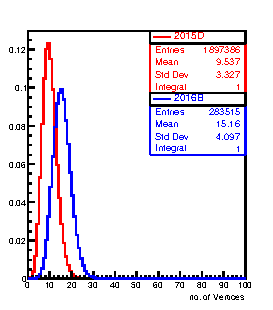
\includegraphics[width=0.99\linewidth]{../Figures/Chap2/ImageFiles_HF/BasicPics/Comp2015vs2016B/nVtx2015D_2016B.pdf}
\captionsetup{width=.9\linewidth}
\caption{Number of primary vertices before re-weighting}
\label{nVtx2015D_2016B}
\end{minipage}
\hspace{0.5cm}
\begin{minipage}[b]{0.5\linewidth}
\centering
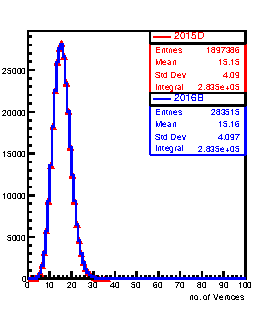
\includegraphics[width=0.99\linewidth]{../Figures/Chap2/ImageFiles_HF/BasicPics/Comp2015vs2016B/nVtx2015DPUwt_2016B.pdf}
\captionsetup{width=.9\linewidth}
\caption{Number of primary vertices after re-weighting}
\label{nVtx2015DPUwt_2016B}
\end{minipage}
\end{figure}

In order to compare the data taken with these different conditions, events had to be rewighted according to the pileup. In this case, number of primary vertices (PV) distribution in 2015D was re-weighted to match PV distribution of 2016B. This was done by simple division of 2016B histogram by 2015D histogram. The resulting histogram gives the pileup weights for 2015D as a function of different PVs. Fig.~\ref{nVtx2015DPUwt_2016B} shows the PV distribution after the reweighing. 
In Fig.~(\ref{nRecHits_2015DPUwt_2016B}-\ref{RecHitES_2015DPUwt_2016B}) some of the HF parameters such as number of RecHits above 10~GeV, RecHit energy in long and short fibers for these runs are compared. These runs show very similar behavior with respect to these parameters.
\begin{figure}[!h]
\begin{minipage}[b]{0.48\linewidth}
\centering
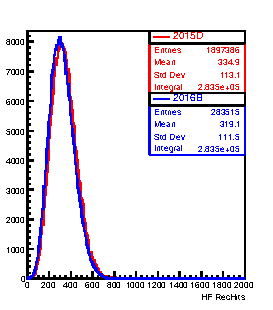
\includegraphics[width=0.9\linewidth]{../Figures/Chap2/ImageFiles_HF/BasicPics/Comp2015vs2016B/nRecHits_2015DPUwt_2016B.pdf}
\captionsetup{width=.9\linewidth}
\caption{No. of HF RecHits above 10 GeV}
\label{nRecHits_2015DPUwt_2016B}
\end{minipage}
%\hspace{0.5cm}
\begin{minipage}[b]{0.48\linewidth}
\centering
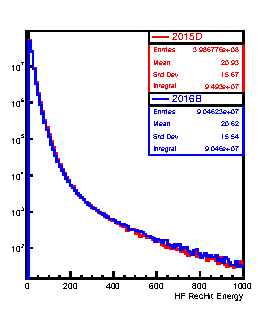
\includegraphics[width=0.9\linewidth]{../Figures/Chap2/ImageFiles_HF/BasicPics/Comp2015vs2016B/RecHitE_2015DPUwt_2016B.pdf}
\captionsetup{width=.9\linewidth}
\caption{HF RecHit energy in long and short fibers}
\label{RecHitE_2015DPUwt_2016B}
\end{minipage}
\end{figure}
\begin{figure}[!h]
\begin{minipage}[b]{0.48\linewidth}
\centering
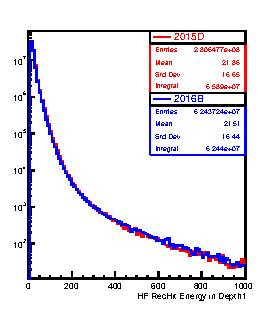
\includegraphics[width=0.99\linewidth]{../Figures/Chap2/ImageFiles_HF/BasicPics/Comp2015vs2016B/RecHitEL_2015DPUwt_2016B.pdf}
\captionsetup{width=.9\linewidth}
\caption{Energy in long}
\label{RecHitEL_2015DPUwt_2016B}
\end{minipage}
%\hspace{1cm}
\begin{minipage}[b]{0.48\linewidth}
\centering
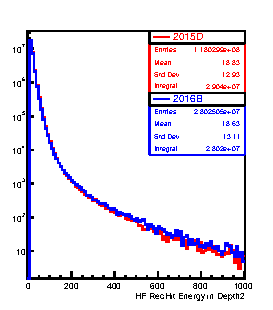
\includegraphics[width=0.99\linewidth]{../Figures/Chap2/ImageFiles_HF/BasicPics/Comp2015vs2016B/RecHitES_2015DPUwt_2016B.pdf}
\captionsetup{width=.9\linewidth}
\caption{Energy in short}
\label{RecHitES_2015DPUwt_2016B}
\end{minipage}
\end{figure}

\ratiosl as a function of different $i\eta$ for 2015 data and 2016B data are compared in Fig.\ref{fig:Ratio2015vs2015B}. The plot shows that both the datasets have similar ratio and the agreement between these datasets is within 1-2\%. It was found that the choice of a different hardonic trigger does not affect \ratiosl features seen in this plot.
\begin{figure}[h!]
\centering
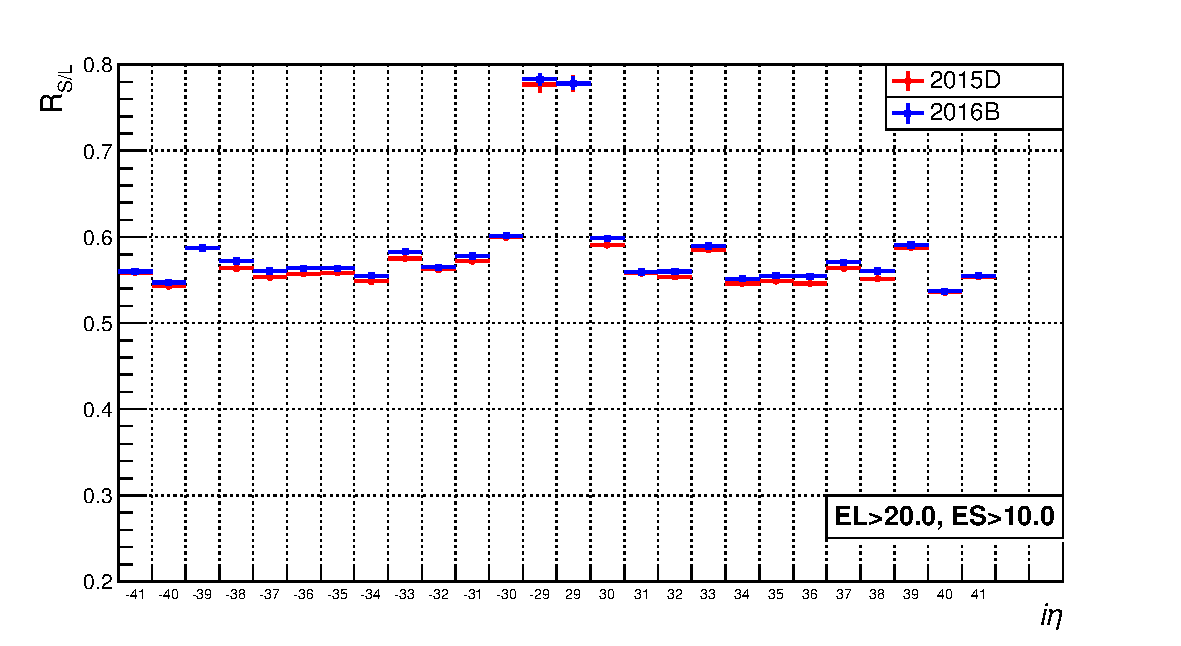
\includegraphics[width=0.7\linewidth]{../Figures/Chap2/ImageFiles_HF/Ratio/2015vs2016/Ratio2015vs2015B}
\caption{\ratiosl for 2015 and 2016B data}
\label{fig:Ratio2015vs2015B}
\end{figure}

\subsection{Performance of \ratiosl in 2016 Data}
In this section, different run eras of 2016 data (era B to H) are compared using JetHT dataset and events with 
at least one jet with $\pt > 450$ \gev at trigger level.
Different run eras of 2016 had different pileup scenarios and 2016B has the 
smallest pileup among these. This can be clearly seen from the distributions 
of number of primary vertices (Fig.~\ref{nVtx2016BtoH}).
 If the pileup is higher, then the number of rechits 
are also higher. So larger pileup runs have higher mean number of rechits as 
shown in Fig.~\ref{nRecHits2016BtoH}. All these distributions are
normalized to unit area.


\begin{figure}[!h] % nVtx2016BtoE and nVtx2016BFGH
%\begin{minipage}[b]{0.5\linewidth} % nVtx2016Bto
\centering
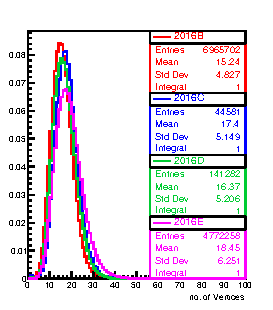
\includegraphics[width=0.45\linewidth]{../Figures/Chap2/ImageFiles_HF/BasicPics/Comp2016/nVtx2016BtoE.pdf}
%\caption{Number of PVs for 2016B,C,D,E}
%\label{nVtx2016BtoE}
%\end{minipage}
%\begin{minipage}[b]{0.5\linewidth} % nVtx2016BFGH
%\centering
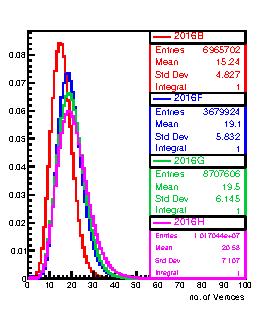
\includegraphics[width=0.45\linewidth]{../Figures/Chap2/ImageFiles_HF/BasicPics/Comp2016/nVtx2016BFGH.pdf}
\caption{Number of primary vertices (left) for 2016B,C,D,E, and (right) for 2016B,F,G,H.}
\label{nVtx2016BtoH}
%\end{minipage}
\end{figure}

\begin{figure}[!h] %nRecHits2016BtoE and nRecHits2016BFGH
%\begin{minipage}[c]{0.5\linewidth}
\centering
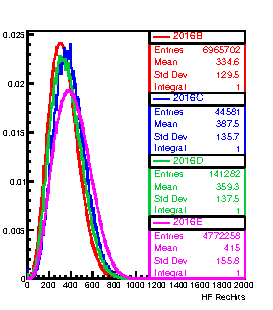
\includegraphics[width=0.45\linewidth]{../Figures/Chap2/ImageFiles_HF/BasicPics/Comp2016/nRecHits2016BtoE.pdf}
%\caption{Number of RecHits for 2016B,C,D,E}
%\label{nRecHits2016BtoE}
%\end{minipage}
%\begin{minipage}[c]{0.5\linewidth}
%\centering
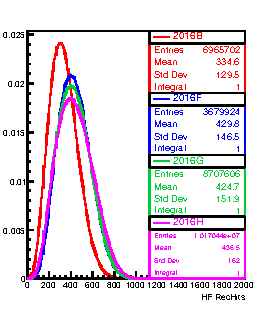
\includegraphics[width=0.45\linewidth]{../Figures/Chap2/ImageFiles_HF/BasicPics/Comp2016/nRecHits2016BFGH.pdf}
\caption{Number of RecHits (left) for 2016B,C,D,E, and (right) for 2016B,F,G,H.}
\label{nRecHits2016BtoH}
%\end{minipage}
\end{figure}

\begin{figure}[!h] %RecHit Energy 2016BtoE
\begin{minipage}[c]{0.32\linewidth}
\centering
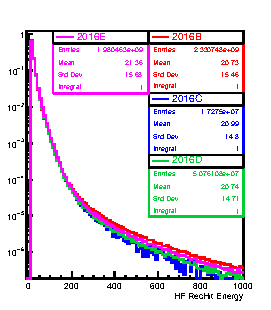
\includegraphics[width=0.99\linewidth]{../Figures/Chap2/ImageFiles_HF/BasicPics/Comp2016/RecHitsE2016BtoE.pdf}
%\caption{RecHitEnergy for 2016B,C,D,E}
%\label{RecHitsE2016BtoE}
\end{minipage}
\begin{minipage}[c]{0.32\linewidth}
\centering
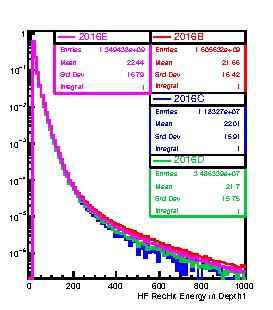
\includegraphics[width=0.99\linewidth]{../Figures/Chap2/ImageFiles_HF/BasicPics/Comp2016/RecHitsEL2016BtoE.pdf}
%\caption{RecHitEnergy in Long}
%\label{RecHitsEL2016BtoE}
\end{minipage}
\begin{minipage}[c]{0.32\linewidth}
\centering
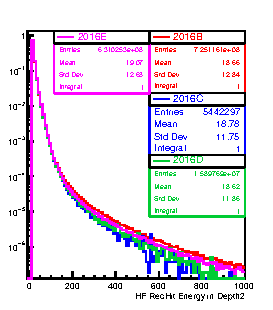
\includegraphics[width=0.99\linewidth]{../Figures/Chap2/ImageFiles_HF/BasicPics/Comp2016/RecHitsES2016BtoE.pdf}
%\caption{RecHitEnergy in Short}
%\label{RecHitsES2016BtoE}
\end{minipage}
\caption{RecHitEnergy distributions for 2016B,C,D,E}
\label{RecHitE2016BtoE}
\end{figure}
\begin{figure}[!h] %RecHit Energy 2016BFGH
\begin{minipage}[c]{0.32\linewidth}
\centering
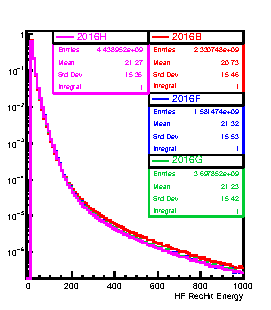
\includegraphics[width=0.99\linewidth]{../Figures/Chap2/ImageFiles_HF/BasicPics/Comp2016/RecHitsE2016BFGH.pdf}
%\caption{RecHitEnergy for 2016B,F,G,H}
%\label{RecHitsE2016BFGH}
\end{minipage}
\begin{minipage}[c]{0.32\linewidth}
\centering
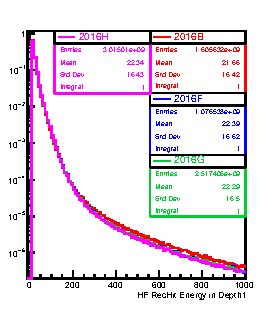
\includegraphics[width=0.99\linewidth]{../Figures/Chap2/ImageFiles_HF/BasicPics/Comp2016/RecHitsEL2016BFGH.pdf}
%\caption{RecHitEnergy in Long}
%\label{RecHitsEL2016BFGH}
\end{minipage}
\begin{minipage}[c]{0.32\linewidth}
\centering
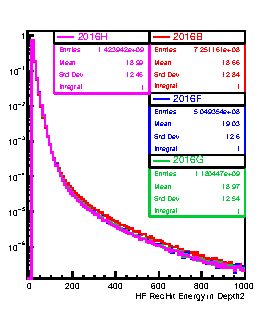
\includegraphics[width=0.99\linewidth]{../Figures/Chap2/ImageFiles_HF/BasicPics/Comp2016/RecHitsES2016BFGH.pdf}
%\caption{RecHitEnergy in Short}
%\label{RecHitsES2016BFGH}
\end{minipage}
\caption{RecHitEnergy distributions for 2016B,F,G, H}
\label{RecHitE2016BFGH}
\end{figure}
RecHit energy distributions for all run eras of 2016 show similar features (Fig.\ref{RecHitE2016BtoE} - \ref{RecHitE2016BFGH}). Any differences seen in these distributions are because of the different pileup scenarios. In case of run 2016C and D, because of lower statistics (only a part of whole dataset was used), energy distributions show small variations. Run 2016B has lower pileup as compared to others and hence, energy distributions are slightly different from other runs. Runs 2016F to 2016H have very similar pileup and hence their energy distributions show better agreement (Fig.\ref{RecHitE2016BFGH}).\\

\subsubsection{Stability of \ratiosl in 2016 Data}
In order to check the stability of \ratiosl across different $i\eta$ channels, mean \ratiosl as a function of $i\eta$ is plotted for all the run eras of 2016 (Fig.\ref{RatioVsIeta2016EL20ES10}). Higher energy thresholds are also used to compare \ratiosl of different run eras across various $i\eta$ channels. Fig.~\ref{RatioVsIeta2016EL50ES10} shows \ratiosl as a function of $i\eta$ with $E_{long}>50~$\gev and $E_{short}>10~$\gev. \ratiosl is found to be stable across all these run eras and also for different energy thresholds.\\
\begin{figure}[h!]%R vs ieta 2016
%\begin{minipage}[c]{0.5\linewidth}
\centering
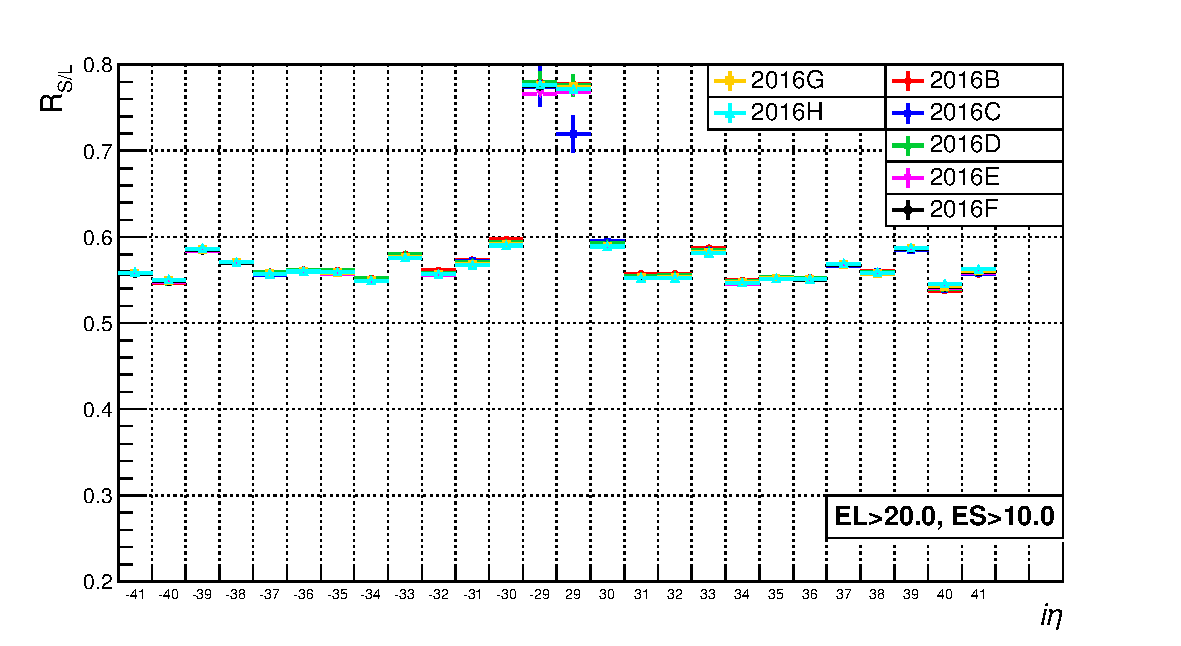
\includegraphics[width=0.8\linewidth]{../Figures/Chap2/ImageFiles_HF/Ratio/2016/RatioVsIeta2016EL20ES10.pdf}
\caption{$\ratiosl$ vs $i\eta$ for 2016 with lower $E_{long}$ threshold}
%\caption{(a)}
\label{RatioVsIeta2016EL20ES10}
%\end{minipage}
\end{figure}
\begin{figure}[h!]%R vs ieta 2016
%\begin{minipage}[c]{0.5\linewidth}
\centering
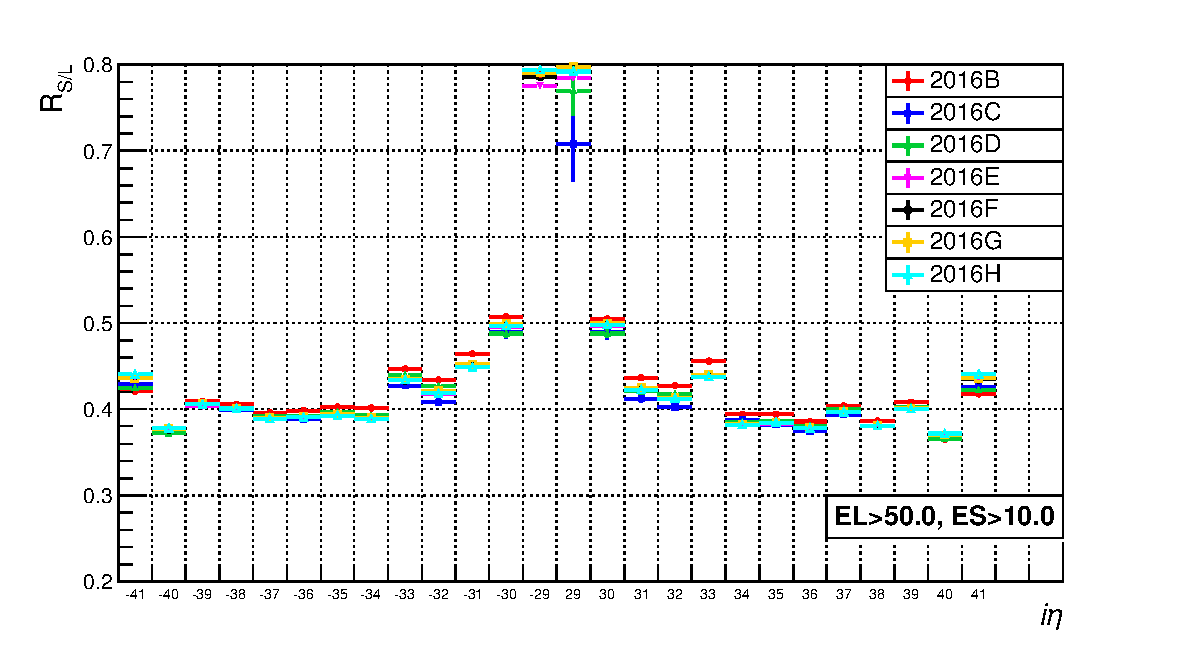
\includegraphics[width=0.8\linewidth]{../Figures/Chap2/ImageFiles_HF/Ratio/2016/RatioVsIeta2016EL50ES10.pdf}
\caption{$\ratiosl$ vs $i\eta$ for 2016 with higher $E_{long}$ threshold}
%\caption{(b)}
\label{RatioVsIeta2016EL50ES10}
%\end{minipage}
%\caption{Mean \ratiosl vs $i\eta$ for 2016 runs with lower (a) and higher (b) $E_{long}$ threshold}
\end{figure}

Corresponding to each $i\eta$ channels, there are 36 divisions in HF. ($|i\eta| = 40,41 $ have 18 divisions). 
\ratiosl as a function of $i\phi$ for a given $i\eta$ channel is also studied and a few such plots are shown
in Fig.\ref{RvsIphiFor2016BtoE} and Fig.\ref{RvsIphiFor2016BFGH}. 
% \textcolor{red}{\ratiosl vs $i\phi$ for all other $i\eta$ are shown in appendix \ref{fig:ieta29_32_E1E2Cut0Ietaiphi2016BtoE} - \ref{fig:ieta41_E1E2Cut0Ietaiphi2016BFGH}.}
Across all the channels for all these run eras, \ratiosl show consistent features. These plots clearly indicate
that \ratiosl is stable across different run eras.\\
To make sure that there is no bias involved in using the JetHT dataset, comparison of \ratiosl for 
JetHT and a dataset consisting of muons (triggered by a muon with $\pt > 50$ \gev)  is done. 
These two datasets showed very similar \ratiosl % \textcolor{red}{and the plot is shown in fig.\ref{fig:2016B2SingMu} appendix A}.
\begin{figure}[!h] %R vs iphi 2016BtoE
\begin{minipage}[c]{0.5\linewidth}
\centering
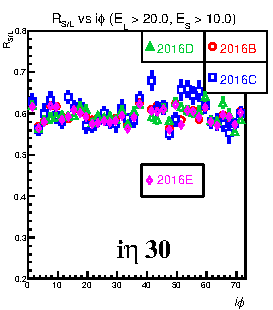
\includegraphics[width=0.7\linewidth]{../Figures/Chap2/ImageFiles_HF/Ratio/2016/ieta30For2016BtoE.pdf}
\end{minipage}
\begin{minipage}[c]{0.5\linewidth}
\centering
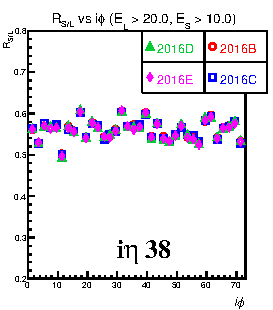
\includegraphics[width=0.7\linewidth]{../Figures/Chap2/ImageFiles_HF/Ratio/2016/ieta38For2016BtoE.pdf}
\end{minipage}
\caption{\ratiosl vs $i\phi$ for 2016B,C,D,E}
\label{RvsIphiFor2016BtoE}
\end{figure}
\begin{figure}[!h] %R vs iphi 2016BFGH
\begin{minipage}[c]{0.5\linewidth}
\centering
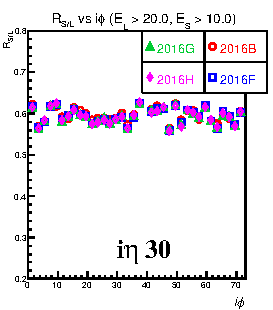
\includegraphics[width=0.7\linewidth]{../Figures/Chap2/ImageFiles_HF/Ratio/2016/ieta30For2016BFGH.pdf}
\end{minipage}
\begin{minipage}[c]{0.5\linewidth}
\centering
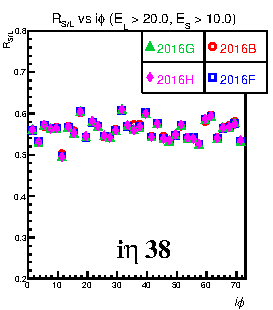
\includegraphics[width=0.7\linewidth]{../Figures/Chap2/ImageFiles_HF/Ratio/2016/ieta38For2016BFGH.pdf}
\end{minipage}
\caption{\ratiosl vs $i\phi$ for 2016B,C,D,E}
\label{RvsIphiFor2016BFGH}
\end{figure}

\subsection{Corrections for the \ratiosl Based on $\phi$ Symmetry}
All the physics processes are symmetric in the azimuthal, $\phi$ direction ( or the transverse x-y plane). 
So \ratiosl is also expected to be symmetric or flat across all $\phi$ channels for a given $\eta$ or $i\eta$.
Based on this symmetry, corrections are derived for the ratio such that \ratiosl is constant across all the $\phi$ channels for a given $\eta$. The corrections are derived as follows:
\begin{itemize}
\item Fit the \ratiosl vs $i\phi$ plot of 2016B with line of 0 slope, and intercept k.
\item Correction for a channel is nothing but original \ratiosl times the intercept.
\end{itemize}
\begin{equation}
Correction(i\eta,i\phi) = k_{i\eta} \times \ratiosl \\
\end{equation}
\begin{equation}
Corrected\ ratio(i\eta,i\phi) = R_{S/L}^{Corr} = Correction(i\eta,i\phi) \times \ratiosl
\end{equation}
These corrections are obtained for all the channels of HF using 2016B dataset with $E_{long} > 50~GeV$ and $E_{Short} > 10~GeV$. The corrections factors as a function of $\eta$ and $i\phi$ are shown in Fig.\ref{fig:corrFacEL50ES10}. 
%These correction factors are also listed in tab.\ref{tab:corrFacPosEta} and tab.\ref{tab:corrFacNegEta} of appendix.
These corrections are applied to 2016B and the remaining 2016 run eras with the same threshold on $E_{long}$ and $E_{Short}$.
 (The errors on the correction factors are dependent on the error on the mean \ratiosl and the fit uncertainty. These errors are less than 1\% for almost all the channels, except for $|i\eta|$=29)
\begin{figure}[h]
\centering
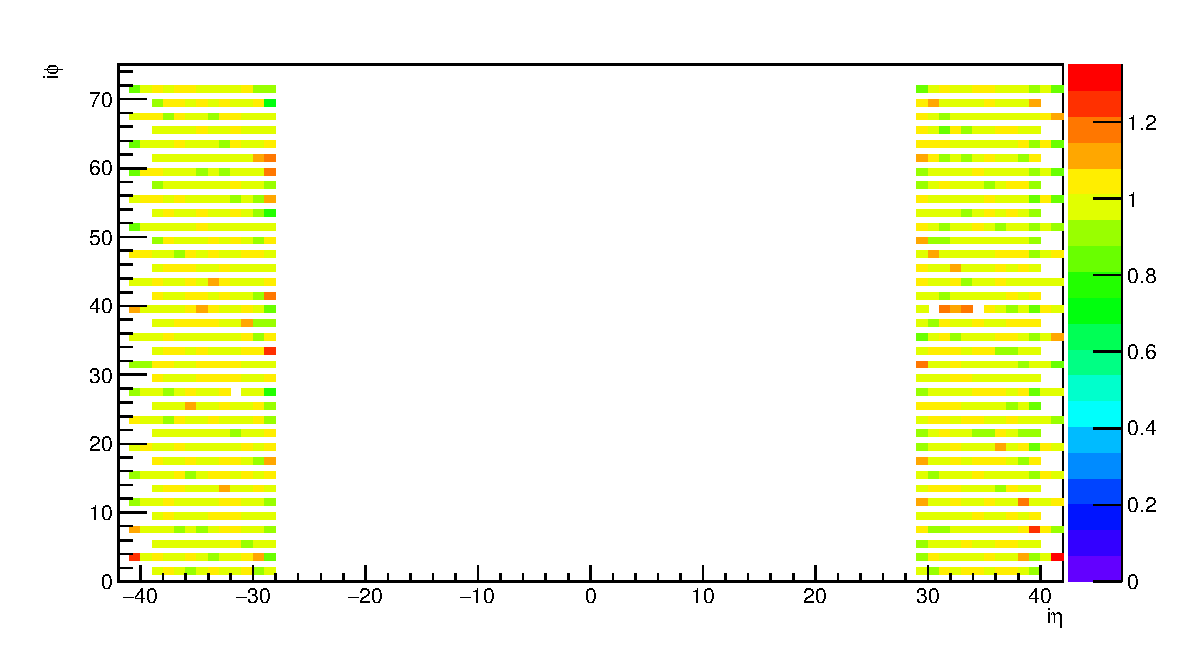
\includegraphics[width=0.7\linewidth]{../Figures/Chap2/ImageFiles_HF/Ratio/2016/corrFacEL50ES10.pdf}
\caption{Correction factors as a function of $i\eta, i\phi$}
\label{fig:corrFacEL50ES10}
\end{figure}

Fig.~\ref{corrected2016BFGH_38} shows the comparison of ratio plots before correction (left)and after correction (right). Similar features are seen for other run eras i.e, 2016C,D and E. %Complete set of plots corresponding to all run eras are shown in appendix Fig.\ref{fig:ieta29_32_E1E2Cut3IetaiphiBtoE} - Fig.\ref{fig:ieta41_E1E2Cut3Ietaiphi_Crrtd}. (2016C and 2016D have low statistics and hence the errors would be large)\\

\begin{figure}[!h] %R corrected vs iphi 2016BFGH
\begin{minipage}[c]{0.5\linewidth}
\centering
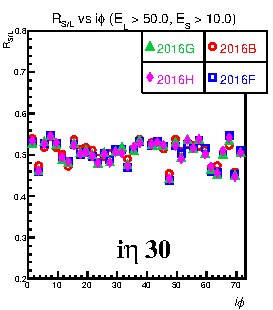
\includegraphics[width=0.7\linewidth]{../Figures/Chap2/ImageFiles_HF/Ratio/2016/Corrected/ieta30Cut3Ietaiphi.pdf}
\end{minipage}
\begin{minipage}[c]{0.5\linewidth}
\centering
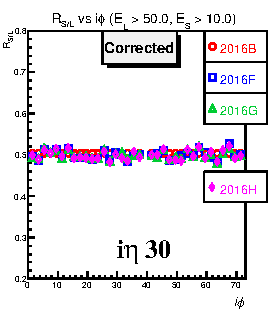
\includegraphics[width=0.7\linewidth]{../Figures/Chap2/ImageFiles_HF/Ratio/2016/Corrected/ieta30Cut3Ietaiphi_corr.pdf}
\end{minipage}
\caption{\ratiosl vs $i\phi$ for $i\eta=$30 for (left) current detector, and (right) after corrections for 2016B,F,G,H}
\label{corrected2016BFGH_30}
\end{figure}

\begin{figure}[!h] %R corrected vs iphi 2016BFGH
\begin{minipage}[c]{0.5\linewidth}
\centering
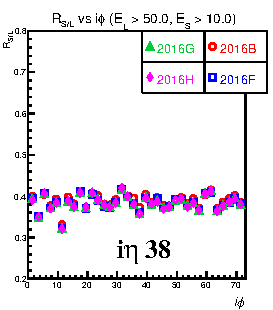
\includegraphics[width=0.7\linewidth]{../Figures/Chap2/ImageFiles_HF/Ratio/2016/Corrected/ieta38Cut3Ietaiphi.pdf}
\end{minipage}
\begin{minipage}[c]{0.5\linewidth}
\centering
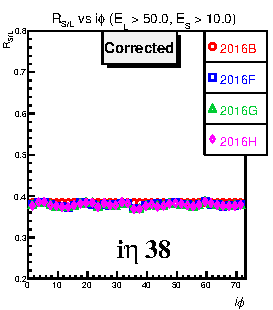
\includegraphics[width=0.7\linewidth]{../Figures/Chap2/ImageFiles_HF/Ratio/2016/Corrected/ieta38Cut3Ietaiphi_corr.pdf}
\end{minipage}
\caption{\ratiosl vs $i\phi$ for $i\eta=$38 for (left) current detector, and (right) after corrections for 2016B,F,G,H}
\label{corrected2016BFGH_38}
\end{figure}
Corrections derived so far had energy threshold on long as 50 GeV and almost no energy threshold on short energy (10 GeV). Using 50 GeV threshold on long makes the corrections less prone to pileup dependencies. To check the dependency of the corrections on energy thresholds used, these corrections are also used for the ratio plots with different thresholds on long for the same dataset 2016B. Fig.~\ref{Ecut1CorrectionEcut3} and \ref{Ecut4CorrectionEcut3} show the ratio plots before and after corrections for the energy thresholds $E_{long} > 30~GeV$ and $E_{long} > 100~GeV$. The corrections are derived from 2016B with $E_{long} > 50~GeV$. The corrected points are multiplied by a factor of 1.3 so that they can be visualized in the same plots. %Fig.~\ref{fig:ieta29_32_E1E2Cut1Ietaiphi_Crrtd} - Fig.~\ref{fig:ieta41_E1E2Cut4Ietaiphi_Crrtd} in appendix shows all the plots corresponding to all $i\eta$ channels with these thresholds.
\begin{figure}[!h] %R corrected vs iphi 2016BFGH Energy
\begin{minipage}[c]{0.5\linewidth}
\centering
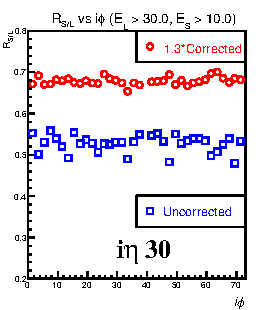
\includegraphics[width=0.7\linewidth]{../Figures/Chap2/ImageFiles_HF/Ratio/2016/Corrected/EnegyCut3010/ieta30Ecut1CorrectionEcut3.pdf}
\end{minipage}
\begin{minipage}[c]{0.5\linewidth}
\centering
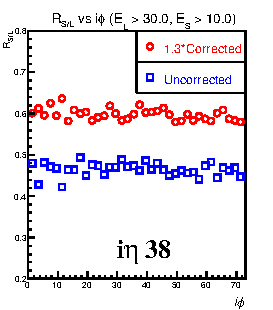
\includegraphics[width=0.7\linewidth]{../Figures/Chap2/ImageFiles_HF/Ratio/2016/Corrected/EnegyCut3010/ieta38Ecut1CorrectionEcut3.pdf}
\end{minipage}
\caption{\ratiosl vs $i\phi$ before and after corrections for 2016B with $E_{long} > 30$, $E_{short} >10$}
\label{Ecut1CorrectionEcut3}
\end{figure}
\begin{figure}[!h] %R corrected vs iphi 2016BFGH Enegy
\begin{minipage}[c]{0.5\linewidth}
\centering
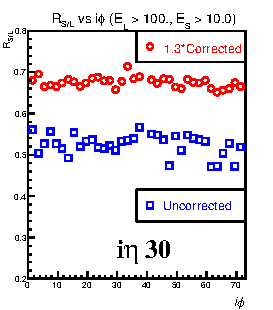
\includegraphics[width=0.7\linewidth]{../Figures/Chap2/ImageFiles_HF/Ratio/2016/Corrected/EnergyCut10010/ieta30Ecut4CorrectionEcut3.pdf}
\end{minipage}
\begin{minipage}[c]{0.5\linewidth}
\centering
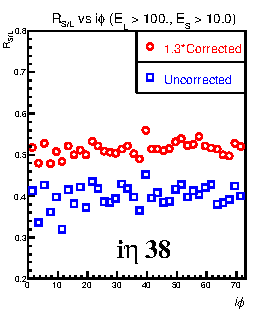
\includegraphics[width=0.7\linewidth]{../Figures/Chap2/ImageFiles_HF/Ratio/2016/Corrected/EnergyCut10010/ieta38Ecut4CorrectionEcut3.pdf}
\end{minipage}
\caption{\ratiosl vs $i\phi$ before and after corrections for 2016B with $E_{long} > 100$, $E_{short} >10$}
\label{Ecut4CorrectionEcut3}
\end{figure}

It is clear from the Fig.\ref{corrected2016BFGH_38}-Fig.\ref{Ecut4CorrectionEcut3} that using the corrections on the ratio, improves the symmetry in $\phi$.\\
The long fibers are be calibrated using $Z\rightarrow e^+ + e^-$ events. The plots shown indicate that \ratiosl is stable across different runs and it improves the $\phi$ symmetry. So \ratiosl can be used as a tool to inter-calibrate the short fibers.


\subsection{Performance of \ratiosl in data \& MC}\label{sec:ana25ns}
In this section comparison of QCD MC sample with data is done. JetHT dataset of 2016E is used for the studies. Trigger used to select events in the data is found to be $\approx 100\%$ efficient for jet $p^T>500~$GeV. There is no trigger requirement for the MC samples. Apart from this selection, the event must contain (in both data and MC) at least one jet with $p^T>600~$GeV and within $|\eta|<2.4$. Nominal HF rechit filters are also used.\\
Data and MC have different number of observed interactions or different pileup (Fig.\ref{fig:DataMCobsIntPUWt}). So MC is re-weighted such that the observed number of interactions in data and MC match. 
Solid blue line corresponds to the observed interactions in MC before PU re-weighting and dotted blue refers to observed interactions in MC after PU re-weighting.\\
MC is scaled to integrated luminosity of the data ($=4.05\ \fbinv$). After this scaling of MC, MC had more events (integral) than data (about 20\% higher). So MC is scaled down so that the integrals in data and MC match. 

\begin{figure}[h!]
\centering
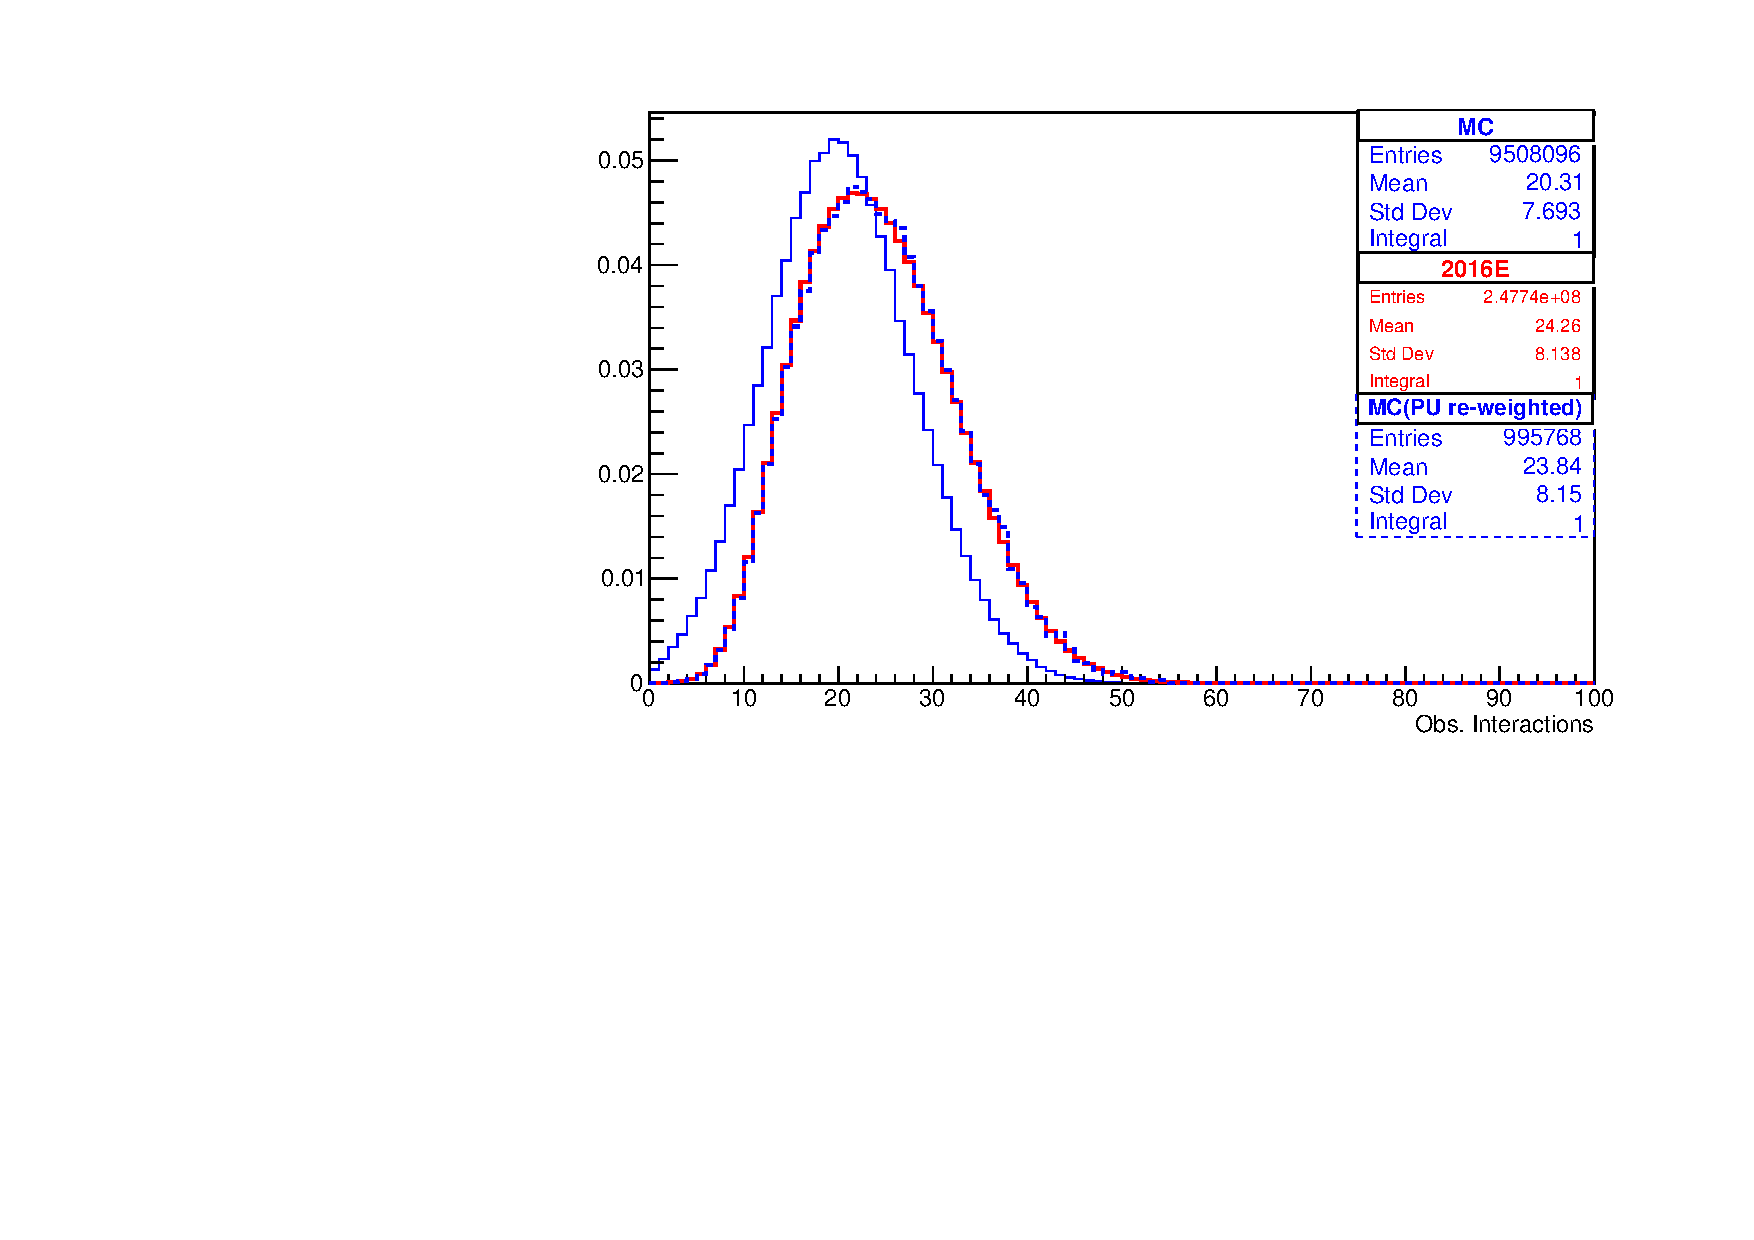
\includegraphics[width=0.7\linewidth]{../Figures/Chap2/ImageFiles_HF/BasicPics/DataMC/DataMCobsIntPUWt}
\captionsetup{width=.9\linewidth}
\caption{Observed number of interactions in data and MC (Solid blue line- MC before PU re-weighting, dotted blue-after PU re-weighting).}
\label{fig:DataMCobsIntPUWt}
\end{figure}
Fig.~\ref{fig:nVtxDataMC} shows the number of reconstructed primary vertices and Fig.~\ref{fig:nRecHitsDataMC} shows the number of HF rechits above 10 GeV (after all MC re-weightings mentioned above).

\begin{figure}[h!]
\begin{minipage}[c]{0.5\linewidth}
\centering
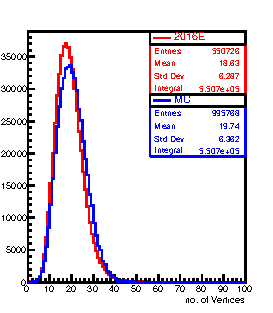
\includegraphics[width=0.9\linewidth]{../Figures/Chap2/ImageFiles_HF/BasicPics/DataMC/nVtxDataMC}
\captionsetup{width=.9\linewidth}
\caption{Number of reconstructed primary vertices in data and MC}
\label{fig:nVtxDataMC}
\end{minipage}
\begin{minipage}[c]{0.5\linewidth}
\centering
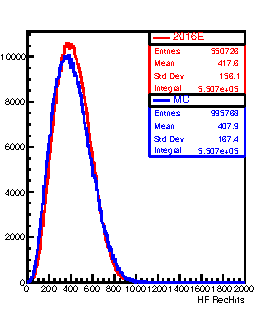
\includegraphics[width=0.9\linewidth]{../Figures/Chap2/ImageFiles_HF/BasicPics/DataMC/nRecHitsDataMC}
\captionsetup{width=.9\linewidth}
\caption{Number of HF rechits above 10 GeV}
\label{fig:nRecHitsDataMC}
\end{minipage}
\end{figure}

\begin{figure}[h!]
%\begin{minipage}[c]{0.32\linewidth}
%\centering
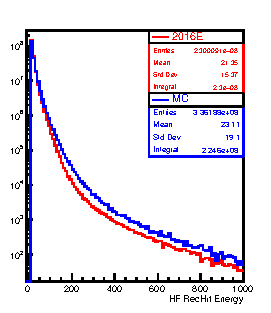
\includegraphics[width=0.32\textwidth]{../Figures/Chap2/ImageFiles_HF/BasicPics/DataMC/HFEnergyDataMC}
%\caption{HF rechit energy distribution}
%\label{fig:HFEnergyDataMC}
%\end{minipage}
%\begin{minipage}[c]{0.329\linewidth}
%\centering
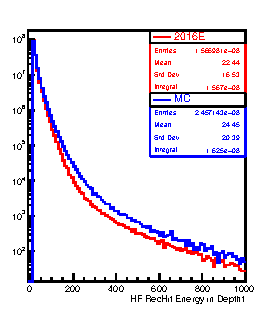
\includegraphics[width=0.32\textwidth]{../Figures/Chap2/ImageFiles_HF/BasicPics/DataMC/ELDataMC}
%\caption{Energy in long(depth1)}
%\label{fig:ELDataMC}
%\end{minipage}
%\begin{minipage}[c]{0.32\linewidth}
%\centering
\includegraphics[width=0.32\textwidth]{../Figures/Chap2/ImageFiles_HF/BasicPics/DataMC/ESDataMC}
\caption{Distribution of energies in (left) all HF rechits, (middle) long fibers or depth\,1, and (right) in short fibers or depth\,2.}
%\label{fig:ESDataMC}
%\end{minipage}
\label{fig:HFEnergyDataMC}
\end{figure}

Fig.~\ref{fig:HFEnergyDataMC} (left) shows the energy distribution in HF. The energy distributions in data and MC show different behavior. Fig.~\ref{fig:HFEnergyDataMC} (middle) shows energy in long and fig.\ref{fig:HFEnergyDataMC} (right) shows the energy in short. The energy distributions in long fibers show more discrepancies as compared to the ones in short. In data, energy falls more rapidly than the ones shown by MC.

\subsubsection{$ \ratiosl$ vs $i\eta$}
Average \ratiosl is determined for data and MC with different energy thresholds on $E_{long}$ and $E_{short}$ and they are plotted as a function of $i\eta$ (Fig.~\ref{fig:DataMCRIeta2010} - Fig.~\ref{fig:DataMCRIeta10010}). If the energy threshold is low (Fig.~\ref{fig:DataMCRIeta2010}), data and MC show large discrepancies. If  higher $E_{long}$ threshold is used, then the agreement is better (Fig.~\ref{fig:DataMCRIeta4010}). However increasing the $E_{long}$ threshold to very high values also shows discrepancies (Fig.~\ref{fig:DataMCRIeta10010}). Increasing short energy threshold along with long threshold gives better agreement (Fig.~\ref{fig:DataMCRIeta5050}) between data and MC. The differences are present at long and short energy itself (Fig.~\ref{fig:HFEnergyDataMC}). If data and MC agree for certain thresholds, then it because the differences in long and short cancel to some extent.\\
As the energy thresholds are varied, shape of the distributions in these plots also change. One reason is that, shape of \ratiosl distribution is different for different $i\eta$ (fig.\ref{goodfit} and fig.\ref{badfit}). The other reason is because of the correlation between long and short energies. Any threshold on long or short affects the energy in the other. In fig.\ref{fig:DataMCRIeta5050}, the threshold on long and short are same (50GeV). This energy threshold will not select many of EM showers since $E_{short}$ is very high. In other words, different thresholds select different EM and hadronic components.

\begin{figure}[h!]
\centering
\includegraphics[width=0.6\linewidth]{../Figures/Chap2/ImageFiles_HF/Ratio/DataMC/DataMCRIeta2010}
\caption{\ratiosl vs $|i\eta|$ with $E_{long}>20,E_{short}>10$ GeV}
\label{fig:DataMCRIeta2010}
\end{figure}
\begin{figure}[h!]
\centering
\includegraphics[width=0.6\linewidth]{../Figures/Chap2/ImageFiles_HF/Ratio/DataMC/DataMCRIeta4010}
\caption{\ratiosl vs $|i\eta|$ with $E_{long}>40,E_{short}>10$ GeV}
\label{fig:DataMCRIeta4010}
\end{figure}

\begin{figure}[h!]
\centering
\includegraphics[width=0.6\linewidth]{../Figures/Chap2/ImageFiles_HF/Ratio/DataMC/DataMCRIeta10010}
\caption{\ratiosl vs $i\eta$ with $E_{long}>100,E_{short}>10$}
\label{fig:DataMCRIeta10010}
\end{figure}

\begin{figure}[h!]
\centering
\includegraphics[width=0.6\linewidth]{../Figures/Chap2/ImageFiles_HF/Ratio/DataMC/DataMCRIeta5050}
\caption{\ratiosl vs $i\eta$ with $E_{long}>50,E_{short}>50$}
\label{fig:DataMCRIeta5050}
\end{figure}

\subsubsection{$ \ratiosl$ vs $i\phi$}
Since \ratiosl vs $i\eta$ plots for data and MC show differences, it is obvious that \ratiosl does not agree for different $i\phi$s as well (Fig.~\ref{fig:RatioVsIphiDataMC}). However, it can be seen that \ratiosl is flat (constant across all $i\phi$) for a given $i\eta$.
\begin{figure}[h!]
%\begin{minipage}[c]{0.5\linewidth}
\centering
\includegraphics[width=0.45\linewidth]{../Figures/Chap2/ImageFiles_HF/Ratio/DataMC/ieta30_E1E2Cut3Ietaiphi}
%\caption{}
%\label{fig:ieta30_E1E2Cut3Ietaiphi}
%\end{minipage}
%\begin{minipage}[c]{0.5\linewidth}
%\centering
\includegraphics[width=0.45\linewidth]{../Figures/Chap2/ImageFiles_HF/Ratio/DataMC/ieta38_E1E2Cut3Ietaiphi}
%\caption{}
%\label{fig:ieta38_E1E2Cut3Ietaiphi}
%\end{minipage}
\caption{\ratiosl vs $i\phi$ for data and MC}
\label{fig:RatioVsIphiDataMC}
\end{figure}

\subsection{Summary of HF studies using \ratiosl}
Study of performance of hadron forward (HF) calorimeter was done using ratio of energy deposited in short to long fibers (\ratiosl) of HF. Data collected by CMS in 2012 with $\sqrt{s}=13$TeV was compared with 2015 data using \ratiosl. For most of the $i\eta$ towers, 2012 showed lower \ratiosl than 2015, which might be because of increased $\sqrt{s}$ or radiation damage. Affect of pileup on \ratiosl was studied and with increased pileup, \ratiosl was found to decrease. Comparison of 25ns bunch spacing 2015 data and 2016 data was done and \ratiosl showed similar features. Different run eras of 2016 also showed similar \ratiosl, which indicates the stability of \ratiosl across these run eras. For a given $i\eta$, different $i\phi$s showed small variations in \ratiosl. Corrections were obtained using 2016B to make the \ratiosl constant (flat) across these $\phi$ channels and these corrections improved flatness of \ratiosl. Assuming that long fibers are well calibrated within a given $i\eta$, these corrections can be used intercalibrate short fibers. Comparison of data and MC was also done and these shows differences in terms of energy distribution in long and short fibers. \ratiosl also shows differences for many of the channels. The agreement in terms of \ratiosl is better for higher enrgy threholds.





